% !TEX program = pdflatex

\documentclass[12pt]{support/thcolognereport} 

\usepackage{amssymb}

\title{Masterthesis: Optimization of Augmented Reality Applications considering the Depth Information with Googles Project Tango}

\degree{Technical Report}

\author{Steffen Tröster}

\college{Cologne University of Applied Sciences}

\company{inovex GmbH}  

\firstExaminer{Prof. Dr. Hubert Randerath}
\firstExaminerLocation{Technische Hochschule Köln}
\secondExaminer{Prof. Dr. Martin Eisemann}
\secondExaminerLocation{Technische Hochschule Köln}

\degreedate{Cologne, \monthyeardate\today}
	
\begin{document}

\baselineskip=18pt plus1pt

\maketitle 

\setlength{\parskip}{1em}

Project Tango is a new mobile platform by Google’s Advanced Technology and Projects (ATAP) team which brings motion tracking, depth perception, and area learning to smartphones and tablets. This technology can be used to realize real world measurement applications, indoor navigation and virtual reality environments.  With its motion tracking technology, Project Tango is also suitable for precise three dimensional augmented reality (AR) applications. The illusion in those applications can be realized by equating the extrinsic and intrinsic camera properties of the real and the virtual camera in a virtual scene. Motion tracking can then be used to update the virtual camera location and orientation continuously. But the illusion of the model projection in these AR applications is often disrupted when real objects in the scene are located in front of virtual projections, that are not getting occluded.

The presented thesis is focusing on this augmented reality problem and is comparing three occlusion mechanisms which can solve the virtual object occlusion with Project Tangos depth perception on mobile hardware and in real time. The idea of real world occlusion by the determined depth information was first introduced by \citet{wloka1995resolving}. They used the z-buffer algorithm and a depth estimation with stereo cameras to prevent a rendering of virtual object parts which are occluded by real object depth information. The presented thesis is indicating three different approaches to fill the z-buffer with depth information captured by the infrared laser sensor, which is integrated in the Project Tango device. It is filled by the direct sensor data projection, by a TSDF based reconstruction called Chisel by \citet{Klingensmith_2015_7924} or by a self combined and implemented plane based reconstruction. 

Project Tango is not producing a depth map which could be integrated into the z-buffer directly. It instead is giving a pointcloud with depth information of the current camera perspective. The first naive and already mentioned approach is the projection of the pointcloud to an image plane which then can be used as z-buffer. The depth sensor is limited to a range of \(50cm\) to \(4m\) and it also has issues capturing depth of complex or reflecting surfaces. Another limitation is the reception rate of only \(5Hz\). Each of these issues is influencing the pointcloud projection due to noise and latency.

\citet{breen1996interactive} are mentioning that the z-buffer based occlusion can also be realized by rendering a primitive based reconstruction as a depth map. Therefore the second approach for solving the mentioned problems, is a plane based reconstruction which was developed during this thesis. It relies on the RANSAC plane estimation from pointclouds by \citet{yang2010plane} and on the plane augmentation and plane range determination method which is used in a SLAM method by \citet{trevor2012planar}. In this approach all incoming points of the depth sensor get collected into an octree with a limited depth for spatial clustering. Then, the RANSAC algorithm is applied to all clusters with new points. It either augments existing planes in this cluster or creates new planes with a limit of three planes per cluster. The reach of each plane is calculated and triangulated by the convex hull. 

The second reconstruction and third depth generating approach of this thesis is based on the real time reconstruction field of research. Unlike to offline reconstruction methods like the Poisson reconstruction by \citet{kazhdan2006poisson} or the approach of \citet{hoppe1992surface}, the challenge for real time reconstruction methods is the migration of continuous depth information from different perspectives into a single augmenting model. \citet{Klingensmith_2015_7924} have presented a real time reconstruction method based on truncated signed distance functions (TSDF) focusing on the mobile application as CPU implementation called Chisel. In this TSDF approach the world is divided into voxel which contain the shortest distance to the next surface. Usually, this representation is rendered via raycasting on desktop environments like in KinectFusion by \citet{newcombe2011kinectfusion}. But \citet{Klingensmith_2015_7924} are using the marching cubes method to get a polygon based representation of the surface. They also integrate a spatial hash data structure presented by \citet{niessner2013real} to minimize the footprint of Chisel for mobile devices.

All theses depth map generating approaches producing errors because of noise and limitations in cluster or voxel sizes. Also the plane based reconstruction is producing gaps between planes, which lead to missing depth information in the depth map. Therefore, a guided filtering approach by \citet{he2010guided} is applied to the depth map. This filter can interpolate the depth according to the edges of the current color image frame captured by the Project Tango device. 

\begin{figure}[h]
  \centering
	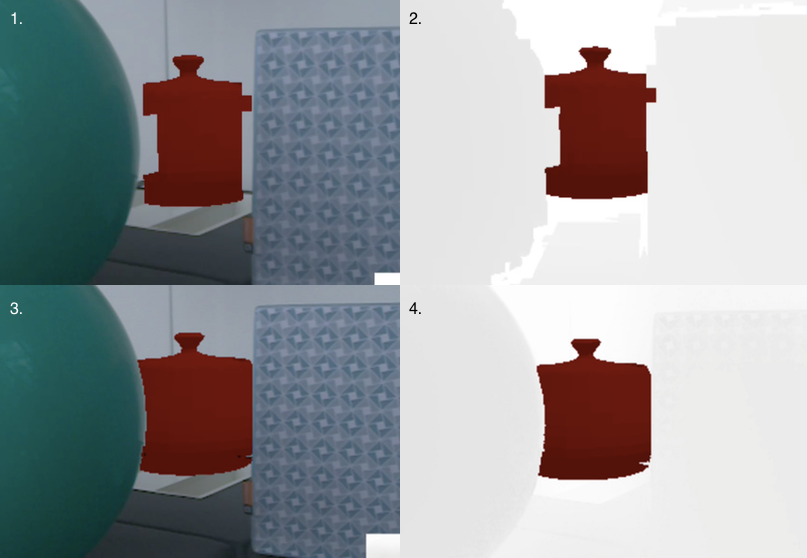
\includegraphics[width=0.7\textwidth]{content/images/report-demo.png} 
  \caption{Protoype Screenshots - (1.) Occlusion by the Chisel Reconstruction (2.) Chisel Reconstruction Depth Map (3.) Guided Filter Result Occlusion (4.) Guided Filter Depth Map}
  \label{fig:filter-demo}
\end{figure}

During this thesis, all mentioned approaches where implemented or ported to the Project Tango development kit as a proof of concept. The final implemented prototype is containing all depth generating approaches and also the guided filter which can be combined and manipulated dynamically for an evaluation purpose. It is written in C++ and is using OpenGL and OpenCV for the rendering and filtering. The final prototype is shown in figure \ref{fig:filter-demo} and is here rendering a scene which was used during the evaluation. Each combination was tested on this static and reproducible setup next to another more complex test setup to ensure the same input information for each tested approach. In addition, some not measurable dynamic tests have been performed to get an impression how the different approaches can be used in production.

All those mentioned six approaches (three depth map generating methods combined with the guided filter) can be used to achieve an augmented reality occlusion by real objects. The naive pointcloud projection has the already mentioned disadvantages of noise and the limited depth range because of sensor limitations. Noise can be successfully reduced by the guided filter which, however, is limited to \(2-3Hz\) due to the OpenCV CPU image processing. Nevertheless, in combination the pointcloud projection could be used for more detailed but size constrained AR scenes. 

The guided filter is also able to close the depth gaps of the developed plane based reconstruction. Although the plane based reconstruction was producing good results in the static tests, it is still rebuilding non-planar surfaces with rough plane approximations. This leads to bigger depth map errors in a more dynamic augmented reality scene where the camera position is not constrained. The cluster size also cannot be reduced, otherwise the RANSAC plane detection would produce statistically more false positives because of less measurement results inside each cluster. 

Good results could be achieved by using the TSDF reconstruction Chisel as seen in figure \ref{fig:filter-demo}. Although the voxel resolution was quite rough in this prototype, this reconstruction system could still be implemented on the GPU, whereby it would benefit on the parallel processing characteristics. By negotiating the reconstruction scale, voxel resolution and performance, the voxel resolution could be still reduced to the limits of the depth sensor.

The guided filter was always able to improve the quality of the real world occlusion in the static scenes. However, some artifacts where observed during the dynamic testing. When an edge in the color frame was just painted on a flat real world surface, which produced also a flat depth map, the filter was alternating the depth map with some artifacts caused by the underlying color structure. This should be investigated next to alternative depth map upsampling methods for mobile usage in future work, like the approach of \citet{Ferstl_2013_ICCV}. Another future idea could be the integration of the guided filter into the OpenGL fragmentshader. This would make the OpenCV binding superfluous and could save the conversion time. The filter would also benefit from the parallel GPU computing characteristics implemented in OpenGL and would run much faster than in this prototype realization. 

Since Lenovo is announcing a cooperation\footnote{Lenovo News - \url{http://goo.gl/jFLNyn} (21.03.16)} with Google, Project Tango promises to get the standardization for motion tracking, depth perception and area learning on mobile devices. Lenovo will publish the first consumer hardware in summer 2016 with Google's Project Tango hard and software. Intel is cooperating\footnote{Intel\textregistered RealSense\textsuperscript{TM} Developer Kits - \url{http://goo.gl/j4Y18A} (21.03.16)} with Google as well and enables his competitive product RealSense\textsuperscript{TM} to run Project Tango applications.

\setlength{\parskip}{0em}

\addcontentsline{toc}{chapter}{References}

\bibliography{main}
\bibliographystyle{apalike} 

\end{document}

